\begin{figure}[H]
  \centering
  \resizebox{!}{0.22\textheight}{%
  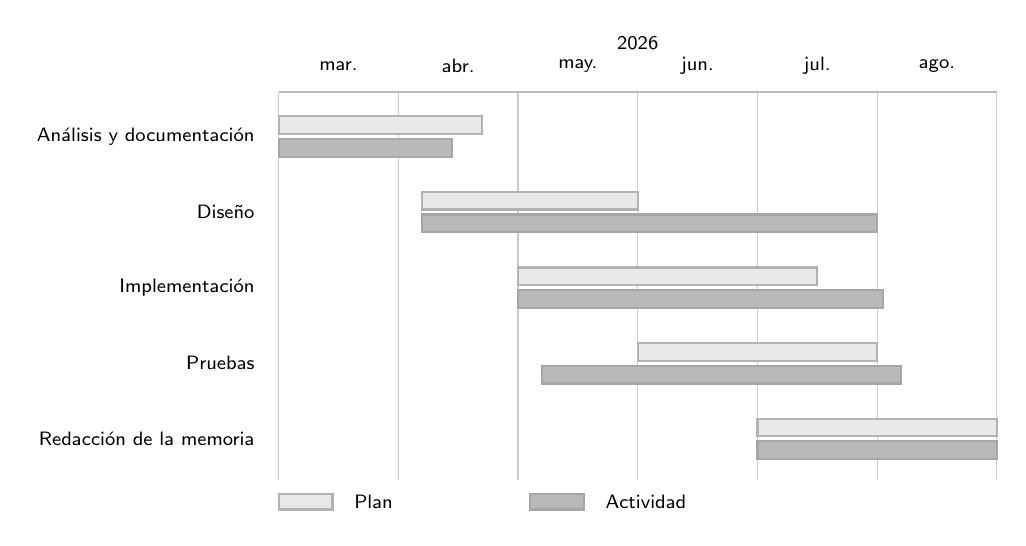
\begin{tikzpicture}[
    x=1.52cm,
    y=-0.32cm,
    font=\footnotesize\sffamily
  ]
    % Rejilla mensual (mar = 0 ... fin de ago = 6)
    \foreach \i in {0,1,2,3,4,5,6} {
      \draw[gray!40] (\i, 1.6) -- (\i, 17.0);
    }
    \draw[gray!55, thick] (0, 1.6) -- (6, 1.6);

    \node[font=\scriptsize\sffamily] at (0.5, 0.55) {mar.};
    \node[font=\scriptsize\sffamily] at (1.5, 0.55) {abr.};
    \node[font=\scriptsize\sffamily] at (2.5, 0.55) {may.};
    \node[font=\scriptsize\sffamily] at (3.5, 0.55) {jun.};
    \node[font=\scriptsize\sffamily] at (4.5, 0.55) {jul.};
    \node[font=\scriptsize\sffamily] at (5.5, 0.55) {ago.};
    \node[font=\scriptsize\sffamily] at (3.0, -0.35) {2026};

    % --- Análisis (plan 0.00--1.70; actividad 0.00--1.45) ---
    \node[anchor=east, align=right, font=\scriptsize\sffamily]
      at (-0.12, 3.35) {Análisis y documentación};
    \fill[gray!18] (0.00, 2.55) rectangle (1.70, 3.25);
    \draw[gray!60, thick] (0.00, 2.55) rectangle (1.70, 3.25);
    \fill[gray!55] (0.00, 3.45) rectangle (1.45, 4.15);
    \draw[gray!70, thick] (0.00, 3.45) rectangle (1.45, 4.15);

    % --- Diseño (plan 1.20--3.00; actividad 1.20--5.00) ---
    \node[anchor=east, font=\scriptsize\sffamily]
      at (-0.12, 6.35) {Diseño};
    \fill[gray!18] (1.20, 5.55) rectangle (3.00, 6.25);
    \draw[gray!60, thick] (1.20, 5.55) rectangle (3.00, 6.25);
    \fill[gray!55] (1.20, 6.45) rectangle (5.00, 7.15);
    \draw[gray!70, thick] (1.20, 6.45) rectangle (5.00, 7.15);

    % --- Implementación (plan 2.00--4.50; actividad 2.00--5.05) ---
    \node[anchor=east, font=\scriptsize\sffamily]
      at (-0.12, 9.35) {Implementación};
    \fill[gray!18] (2.00, 8.55) rectangle (4.50, 9.25);
    \draw[gray!60, thick] (2.00, 8.55) rectangle (4.50, 9.25);
    \fill[gray!55] (2.00, 9.45) rectangle (5.05, 10.15);
    \draw[gray!70, thick] (2.00, 9.45) rectangle (5.05, 10.15);

    % --- Pruebas (plan 3.00--5.00; actividad 2.20--5.20) ---
    \node[anchor=east, font=\scriptsize\sffamily]
      at (-0.12, 12.35) {Pruebas};
    \fill[gray!18] (3.00, 11.55) rectangle (5.00, 12.25);
    \draw[gray!60, thick] (3.00, 11.55) rectangle (5.00, 12.25);
    \fill[gray!55] (2.20, 12.45) rectangle (5.20, 13.15);
    \draw[gray!70, thick] (2.20, 12.45) rectangle (5.20, 13.15);

    % --- Memoria (plan 4.00--6.00; actividad 4.00--6.00) ---
    \node[anchor=east, font=\scriptsize\sffamily]
      at (-0.12, 15.35) {Redacción de la memoria};
    \fill[gray!18] (4.00, 14.55) rectangle (6.00, 15.25);
    \draw[gray!60, thick] (4.00, 14.55) rectangle (6.00, 15.25);
    \fill[gray!55] (4.00, 15.45) rectangle (6.00, 16.15);
    \draw[gray!70, thick] (4.00, 15.45) rectangle (6.00, 16.15);
    % Leyenda
    \fill[gray!18] (0.00, 17.55) rectangle (0.45, 18.15);
    \draw[gray!60, thick] (0.00, 17.55) rectangle (0.45, 18.15);
    \node[anchor=west, font=\scriptsize\sffamily] at (0.55, 17.85) {Plan};
    \fill[gray!55] (2.10, 17.55) rectangle (2.55, 18.15);
    \draw[gray!70, thick] (2.10, 17.55) rectangle (2.55, 18.15);
    \node[anchor=west, font=\scriptsize\sffamily] at (2.65, 17.85)
      {Actividad};
  \end{tikzpicture}%
  }
  \caption{Cronograma del proyecto (marzo--agosto de 2026): barras claras,
  planificación inicial; barras oscuras, actividad ejecutada. La fase de
  pruebas se solapa con la implementación.}
  \label{fig:gantt-inicial}
\end{figure}
